\documentclass{article}
\usepackage{geometry}
 \geometry{
 a4paper,
 total={170mm,250mm},
 left=20mm,
 top=10mm,
 }
\usepackage{graphicx}
\usepackage{float}
\usepackage{enumitem}
\usepackage{caption}
\usepackage{amsmath}
\newcommand*{\addheight}[2][.5ex]{%
  \raisebox{0pt}[\dimexpr\height+(#1)\relax]{#2}%
}
\usepackage{datetime}
\newdate{date}{02}{09}{2016}
\date{\displaydate{date}}
\title{\textbf{Chaotic Dynamics - CSCI 5446} \\
Problem Set 4}
\author{Santhanakrishnan Ramani}
\begin{document}
\maketitle

\section*{Problem 2}
\begin{enumerate}[label=(\alph*)]

\item 
The Figure \ref{fig:prob2a} represents the state-space trajectory emanating from the point $[\theta,\omega] = [3,0.1]$ with \\$m = 0.1kg\,, l = 0.1m\,, \beta = 0\,, \alpha = 0\,, A =0 \,\&\, h = 0.005.$ \par\bigskip
\begin{minipage}{\linewidth}
{
\centering 
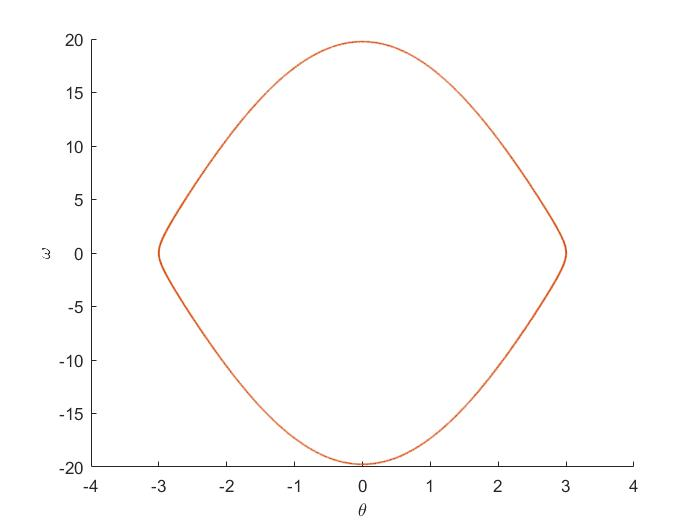
\includegraphics[scale=0.35]{images/prob2a.jpg}
\captionof{figure}{state-space trajectory}
\label{fig:prob2a}
}
\par\medskip
Yes, the initial condition is near the Equilibrium point $[\pi,0]$, and it is unstable.
\end{minipage}
\item
The Figure \ref{fig:prob2b} represents the state-space trajectory emanating from the point $[\theta,\omega] = [0.01,0]$ with \\$m = 0.1kg\,, l = 0.1m\,, \beta = 0\,, \alpha = 0\,, A =0 \,\&\, h = 0.005.$ \par\bigskip
\begin{minipage}{\linewidth}
{
\centering 
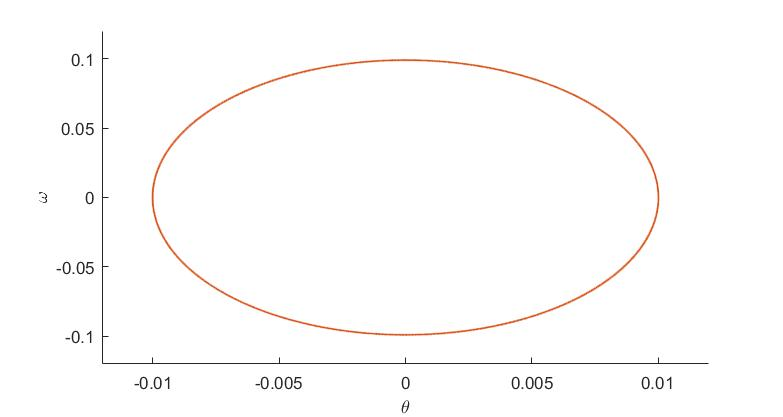
\includegraphics[scale=0.35]{images/prob2b.jpg}
\captionof{figure}{state-space trajectory}
\label{fig:prob2b}
}
\par\medskip
Yes, the trajectory look more like a perfect ellipse than the trajectory of part (a), the reason being the angular velocity is zero, and for smaller angular displacement $\sin(\theta) \approx \theta$, so the rate of change of angular velocity will also be uniform.
\end{minipage}
\end{enumerate}

\section*{Problem 3}
The Figure \ref{fig:prob3} represents the state-space portrait of the system using the coefficient values in Problem 2. \par\bigskip
\begin{minipage}{\linewidth}
{
\centering 
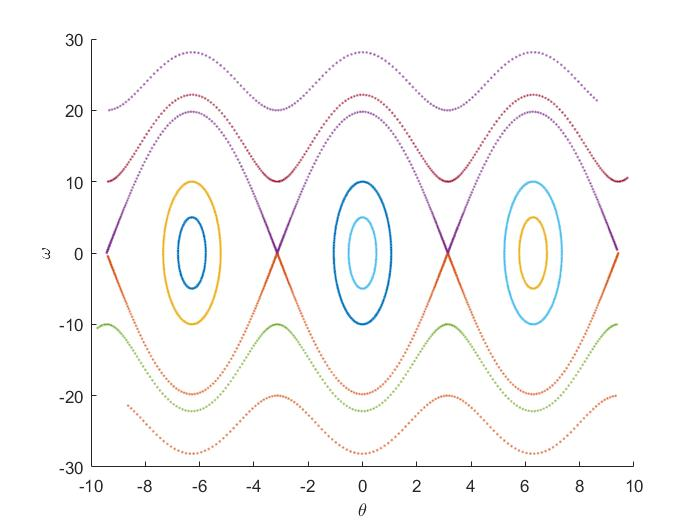
\includegraphics[scale=0.4]{images/prob3.jpg}
\captionof{figure}{state-space portrait}
\label{fig:prob3}
}
\end{minipage}

\section*{Problem 4}
The Figure \ref{fig:prob4} represents the state-space portrait of the system in Problem 3 , excpect the value of $\beta = 0.25$. \\I was able to see the effect of damping clearly affecting the dynamics of the pendulum as it comes to stop by converging to a nearby fixed point after certain rotations which wasn't the case in the previous problem.\par\bigskip
\begin{minipage}{\linewidth}
{
\centering 
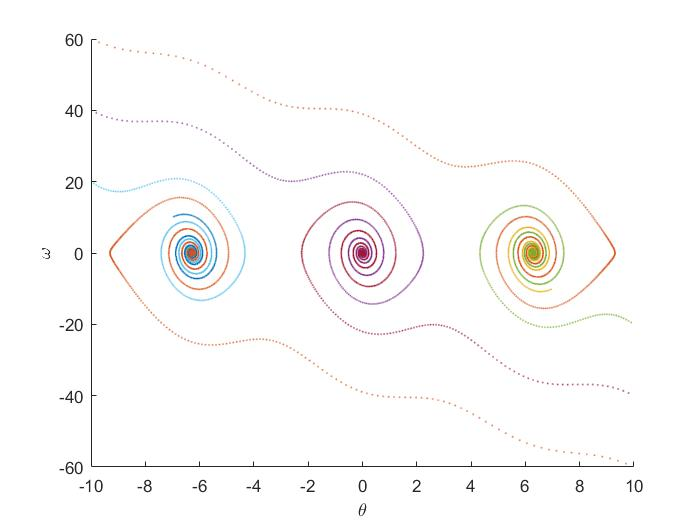
\includegraphics[scale=0.4]{images/prob4.jpg}
\captionof{figure}{state-space portrait}
\label{fig:prob4}
}
\end{minipage}
\par\bigskip
For higher values of $\beta$ the convergence was instant, and for lower values of $\beta$ the converge was seen after few rotations.
\newpage
\section*{Problem 5}
The Figure \ref{fig:prob5} represents the state-space portrait of the system in Problem 4, but plots $\theta\,\, mod\,\, 2\pi$. I was able to see the values starting near the unstable fixed point $[(2n+1)\pi,0]$ converges to a nearby fixed point $[(2n)\pi,0]$ \par\bigskip
\begin{minipage}{\linewidth}
{
\centering 
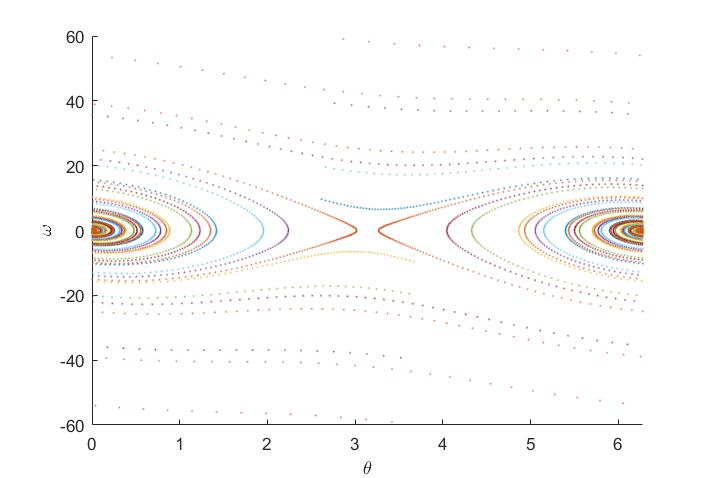
\includegraphics[scale=0.4]{images/prob5.jpg}
\captionof{figure}{state-space portrait}
\label{fig:prob5}
}
\end{minipage}

\section*{Problem 6}
The Figure \ref{fig:prob6} represents a chaotic orbit when $A = 1.1 \,,\, \alpha = 7.4246 \,,\, \beta = 0.25$ \par\bigskip
\begin{minipage}{\linewidth}
{
\centering 
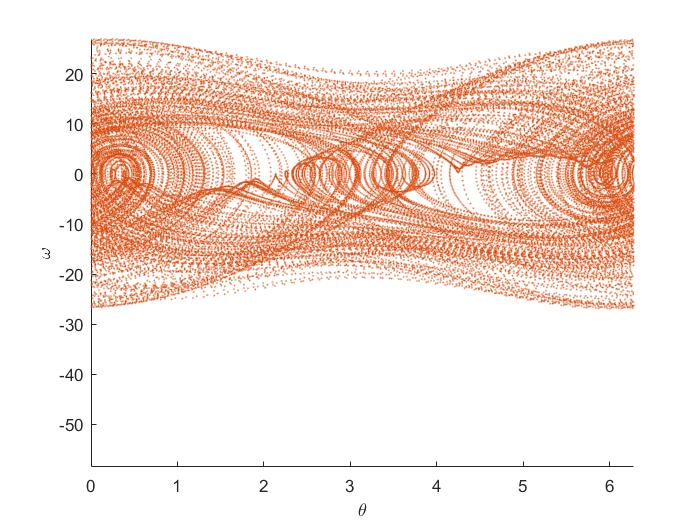
\includegraphics[scale=0.4]{images/prob6.jpg}
\captionof{figure}{state-space portrait}
\label{fig:prob6}
}
\end{minipage}
\par\medskip
As you vary the value of A by increasing it every time by some value you see a pattern of Periodic Orbit and Chaotic Orbit alternating, and each time a Periodic orbit reappears a bifurcation has taken place and there is no symmetry between the periods.

\section*{Problem 7}
\paragraph*{•}
On increasing the value of timeStep by using the values in Problem 2, I found out that it starts to spiral inwards and converge to a fixed stable point initially, and once the value of timeStep is greater than 0.3 it starts to diverge. 
\end{document}
